% Note that the a4paper option is mainly intended so that authors in
% countries using A4 can easily print to A4 and see how their papers will
% look in print - the typesetting of the document will not typically be
% affected with changes in paper size (but the bottom and side margins will).
% Use the testflow package mentioned above to verify correct handling of
% both paper sizes by the user's LaTeX system.
%
% Also note that the "draftcls" or "draftclsnofoot", not "draft", option
% should be used if it is desired that the figures are to be displayed in
% draft mode.
%
\documentclass[journal]{IEEEtran}

\usepackage{cite}
\usepackage[utf8]{inputenc}
\usepackage{siunitx}
\usepackage[pdftex]{graphicx}
\usepackage{mathtools}
\usepackage{bm}
\usepackage{breqn}
\usepackage{enumerate}
\usepackage{listings}
\usepackage{textcomp}
\usepackage[colorlinks=true,urlcolor=blue,linkcolor=red]{hyperref}
\lstset{
  basicstyle=\footnotesize,
  frame = lines
}


% *** MATH PACKAGES ***
%
%\usepackage[cmex10]{amsmath}
% A popular package from the American Mathematical Society that provides
% many useful and powerful commands for dealing with mathematics. If using
% it, be sure to load this package with the cmex10 option to ensure that
% only type 1 fonts will utilized at all point sizes. Without this option,
% it is possible that some math symbols, particularly those within
% footnotes, will be rendered in bitmap form which will result in a
% document that can not be IEEE Xplore compliant!
%
% Also, note that the amsmath package sets \interdisplaylinepenalty to 10000
% thus preventing page breaks from occurring within multiline equations. Use:
%\interdisplaylinepenalty=2500
% after loading amsmath to restore such page breaks as IEEEtran.cls normally
% does. amsmath.sty is already installed on most LaTeX systems. The latest
% version and documentation can be obtained at:
% http://www.ctan.org/tex-archive/macros/latex/required/amslatex/math/


% correct bad hyphenation here
\hyphenation{op-tical net-works semi-conduc-tor matlab}

\newcommand{\vect}[1]{\mathbf{#1}}


\newcommand{\balancecolsandclearpage}{
  \close@column@grid
  \clearpage
  \twocolumngrid
}



\begin{document}

\title{Time Delay Estimation and \\Acoustic Source Localization}

\author{ Javier Ribera Prat }

% The paper headers
\markboth{MATLAB i les seves aplicacions en l'Enginyeria. ETSETB, UPC. \today }
{Shell \MakeLowercase{\textit{et al.}}: Bare Demo of IEEEtran.cls for Journals}
% The only time the second header will appear is for the odd numbered pages
% after the title page when using the twoside option.

\maketitle


\begin{abstract}
  Time Delay Estimation (TDE) is a widely studied research topic which has many applications, specially in target localization and tracking. This article presents a MATLAB implementation and comparison of some algorithms used to do so, with emphasis on their impact on accuracy of the results in an underwater environment. A handy GUI was also developed to assist in visual comparison of algorithms and preprocessing filters. Finally, a simple crossing-lines method was used to try to localize the target. The considered case-study has been a recording from PMRF, an instrumented US Navy testing range located off the island of Kauai, Hawaii. The raw data was collected from seven bottom mounted hydrophones in deep water approximately 45 km northwest of Kauai. Targets were always minke whales.

\end{abstract}

\begin{IEEEkeywords} % Note that keywords are not normally used for peerreview papers.
  TDE, TDOA, localization, tracking, MATLAB, minke whale.
\end{IEEEkeywords}



\section{Introduction}
  % The very first letter is a 2 line initial drop letter followed
% by the rest of the first word in caps.
% 
% form to use if the first word consists of a single letter:
% \IEEEPARstart{A}{demo} file is ....
% 
% form to use if you need the single drop letter followed by
% normal text (unknown if ever used by IEEE):
% \IEEEPARstart{A}{}demo file is ....
% 
% Some journals put the first two words in caps:
% \IEEEPARstart{T}{his demo} file is ....
% 
% Here we have the typical use of a "T" for an initial drop letter
% and "HIS" in caps to complete the first word.
\subsection{Motivation}
  \IEEEPARstart{T}{his} topic was proposed by Ludwig Houégnigan from the \textit{Laboratori d'Aplicacions Bioacústiques} at \textit{Universitat Politècnica de Catalunya} so it can be useful for their research areas.

  The goal is to obtain a solid knowledge of the convenience of some methods used to track the position of cetaceans underwater. Human activities that disrupt marine animal environments such as ships often end up with collisions with cetaceans \cite{collisions}. This leads to injuries and even death for the animals and a danger for sea navigation \cite{youtube-collisions}. Not only vessels in the high seas but also coast cruises face these issues, especially where both whale and ship densities are concentrated. Unfortunately, many incidents of ship strike around the coast go unnoticed or unreported, and this makes it difficult to understand the scope of the problem \cite{web-collisions}.

  Thus, a whale anti-collision system to warn ships in an area about whale locations is required. Moreover, spotting whales positions is also useful for scientific applications such as animal census, behaviour studies, environmental conservation, etc.

\subsection{Scope of the project}
  The following algorithms to compute the TDE have been implemented in MATLAB\footnote{Except simple cross-correlation, for which the simple built-in MATLAB function \emph{xcorr} has been used.}:
  \begin{itemize}
    \item Cross-correlation (CC)
    \item Generalized cross-correlation Phase Transform (GCC-PHAT)
    \item GCC Smoothed Coherence Transform (GCC-SCOT)
    \item Adaptive Least Mean Squares (LMS)
    \item Adaptive Eigenvalue Decomposition (AED)
  \end{itemize}
  \vspace{5pt}
  

  Although, direct use of these algorithms do not yield good results. Hence, some preconditioning methods must be applied previously to the hydrophones recordings. The following filters have also been implemented:
  \begin{itemize}
    \item Pass-band filter
    \item Percentile noise removal
    \item Spectral substraction
    \item Time gain normalization
    \item Teager-Kaiser
  \end{itemize}
  \vspace{5pt}
  
  In addition, a handy straight-forward GUI has been built in order to rapidly compare the algorithms and assess its pros and cons on each kind of signal. Such GUI allows to visually:
  \begin{itemize}
    \item Import a pair of raw \textit{.wav} signals
    \item Select a time segment of this signals in minutes and seconds
    \item Plot their time evolution or spectrogram
    \item Apply any combination of the preprocessing methods
    \item Choose the desired TDE algorithms to assess
    \item Visualize the 3D disposition of the underwater sensors
  \end{itemize}
  \vspace{5pt}

  
\section{Theoretical background}
  \subsubsection{Chosen method}
To estimate the localization of sources, beamforming technique is dismissed in favour of time-delay of arrival (TDOA) method. This is the only feasible method for this case, as beamforming cannot be used when distance between sensors is large. In addition, it is computationally cheaper and uses time signal processing and estimation theory.

TDOA should not be confused with TDE, although here both terms will be used with no distintion. TDE is in general the estimation of the delay of two signals, and can be split in two categories: TOA and TDOA. The former deals with the time difference from the emission of a known signal from the transmitter of a device until the reflection of this signal on the target comes back at the receiver. On the other hand, TDOA tries to estimate the delay of an incoming signal in two separated receivers. This signals is solely produced by the target. As the receivers (in our case hydrophones) are at different positions, the signal that impinges on one sensor would be a shifted version of the one at the other sensor. In this article we will focus on the second case: TDOA. Passive (just listening) is preferable in front of active approaches such as SONAR or beamforming techniques, because of ecological and technical aspects: the microphones used in the available data were separated many kilometers away from each other.

\subsubsection{Cons to face}
The passive TDOA approach and the underwater environment imply some inconvenients that must be taken into consideration:
\begin{enumerate}
  \item The incoming signal is totally unknown, in contrast of in active (TOA) approach, where a simple matched filter would be optimum when the reference signal is produced by us. In our case, TDOA can do no presumption of the waveform, excluding the frequency range. Minke whales usally emit sounds from 1 to \SI{12}{\kilo\Hz}.
  \item Signal to noise ratio (SNR) is very low. This will be the main limitation and that's the reason of the emphasis on the prefiltering methods for noise reduction.
  \item Correlated noise, as the main contribution to it is not white noise, but strong interferences from other animals, devices and water currents.
  \item Reflections on the water surface, mainly. This can make the algorithm to get confused by them and could return a wrong result. Reflections on the seafloor are negligible, as hydrophones are usually placed very near to the ground.
  \item The recordings will not be just a shifted version of the other ones. Noise, reflections and interferences will introduce huge bias and variance in the estimation if not treated correctly.
  \item Sources (whales) will not be still, so delayed will not be a constant in the long-run.
\end{enumerate}

\vspace{5pt}
\subsubsection{Signal model}
  As stated before, the overall results should take into consideration far reflections on the ocean surface. A simple scheme is shown in Figure \ref{fig:reflections}, where flat ground is assumed.  

  \vspace{5pt}
  \begin{figure}[htb]
	  \begin{center}
		  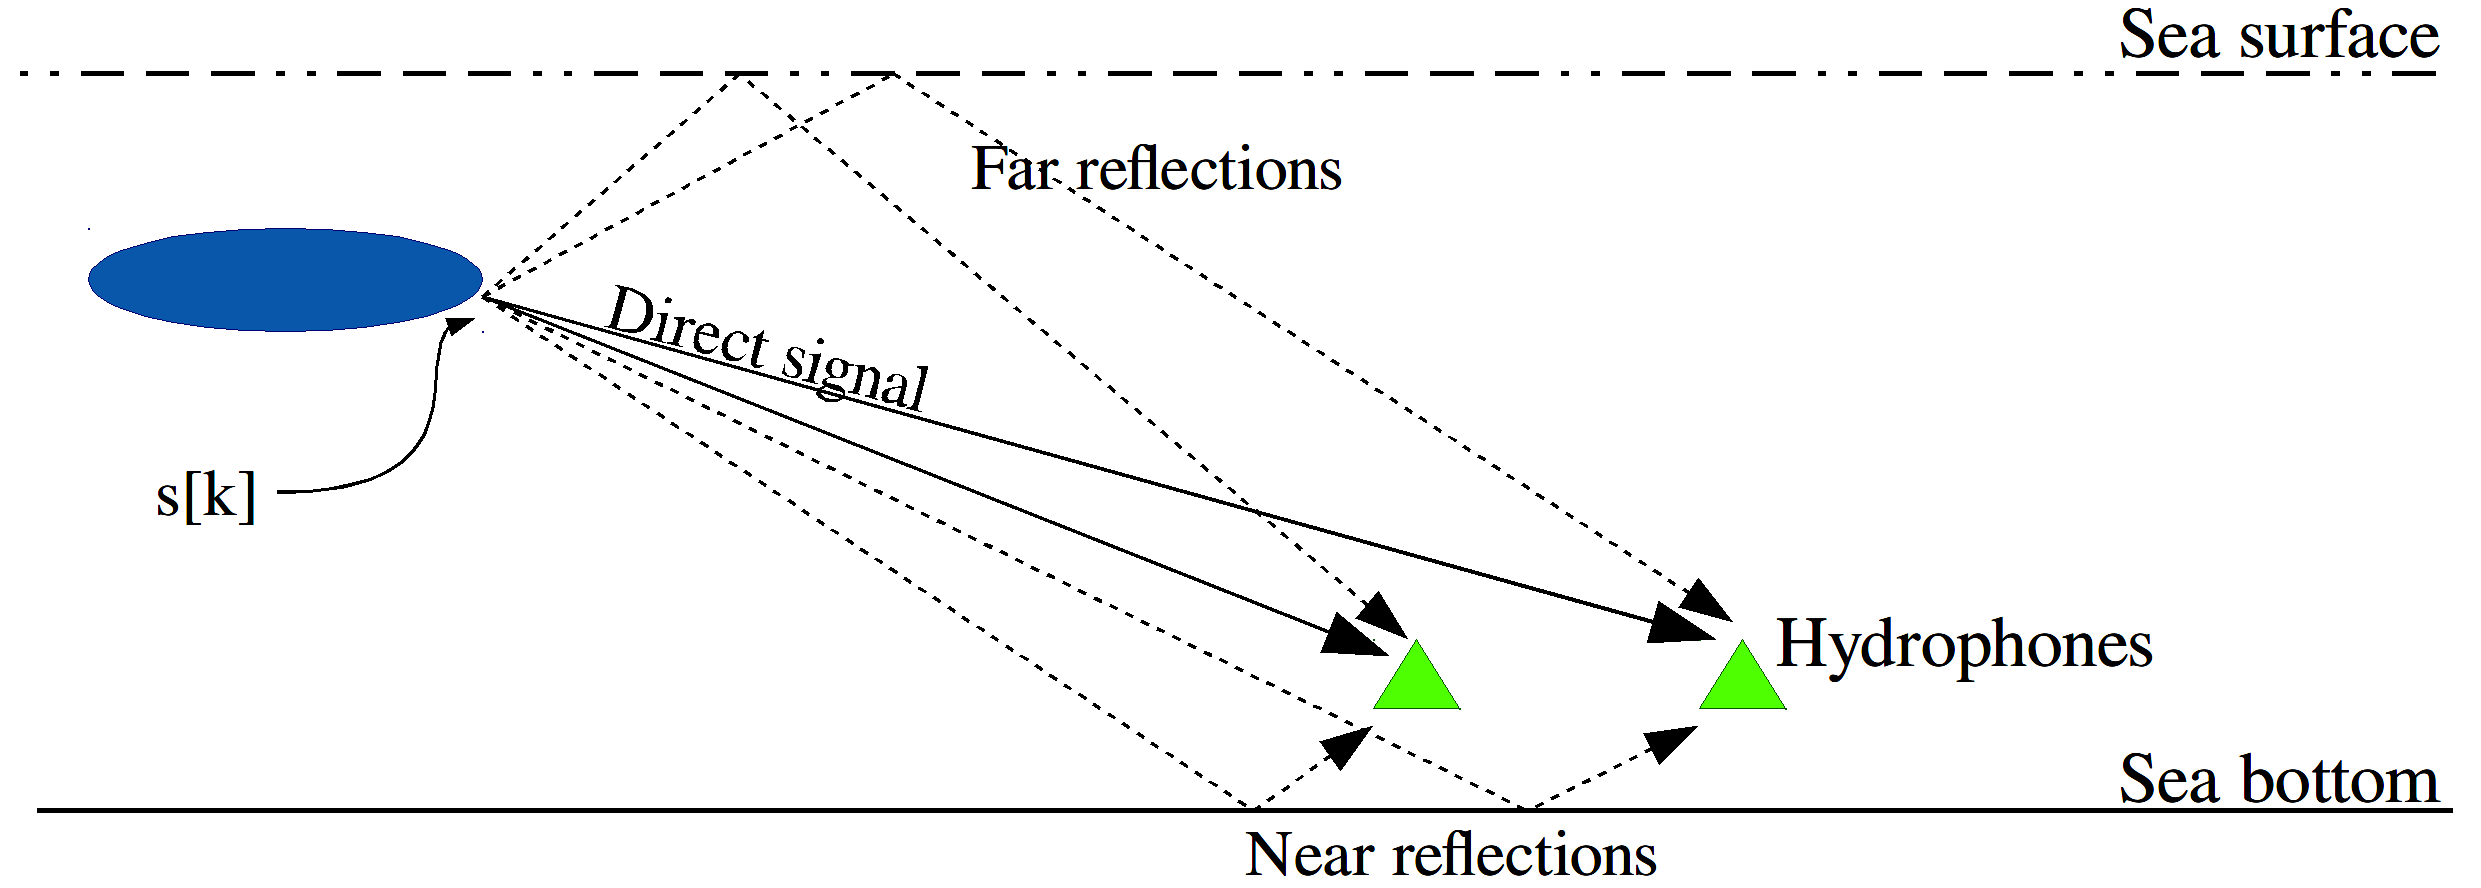
\includegraphics[width=0.5\textwidth]{figures/model.png}
	  \end{center}
	  \caption{Reflections in an underwater environment}
	  \label{fig:reflections}
  \end{figure}
  
  Received signal could be expressed in general as
  $$ r_1[n] = h_1[n]^T s[n] + w_1[n] $$
  $$ r_2[n] = h_2[n]^T s[n] + w_2[n] $$
  
  In an ideal case, $h_k[n]$ would be a Kronecker delta at the delay position, so $h_k[n] = [0\ 0\ ...\ \alpha\ ...\ 0\ 0]$, but in general, as indicated in the last con to face, distorsion and reflections can make the impulse response of the channel to be any kind \cite{overview}.
  $$ h_k[n] = [h_0\ h_1\ ...\ h_{L-1}] $$
  


\section{TDE algorithms}
  In order to get a TDE, some algorithms were developed and a brief explanation of them is shown below:

\subsection{Cross-correlation}
  The cross-correlation function is very simple, so the built-in MATLAB function \emph{xcorr} was used only in this case. For a pair of finite sequences $x_1[n]$ and $x_2[k]$, the maximum of its cross-correlation function $R_{x_1[n] x_2[n]}[m]$ gives the CC TDE:
  \begin{dmath}
    \tau = \arg\max_m R_{x_1[n] x_2[n]}[m]
  \end{dmath}
  
  As MATLAB function \emph{xcorr} returns the result shifted so all values are at positive indexes, the TDE is the difference in samples from the maximum to the middle of the sequence.
  
  This method is the simplest and most straight-forward, but in our scenario it gives the poorest estimations. The code implementation can be seen at file \emph{delay\_xcorr.m}\cite{delayxcorr.m}.
  

\subsection{Generalized cross-correlation}
The generalized cross-correlation (GCC) is a generalization of the cross-correlation in the frequency domain. It is computed as follows:
\begin{dmath}
  R_{GCC_{x_1[n] x_2[n]}}[m] = \text{IFFT}_M\{\Phi[k]S_{x_1x_2}[k]\}[m]
\end{dmath}

Where $S_{x_1x_2}$ is the cross-spectrum of the input signals given by $E\{X_1[k]X^*_2[k]\} $, but for a finite-length sequence it is approximated as $X_1[k]X^*_2[k]$, where $X_j[k]$ denotes the discrete Fourier transform (DFT) of the input signal $x_j[n]$ and $(\cdotp)^*$ the complex conjugate operator.

The function $\Phi[k]$ is the weighting filter. Depending of the chosen weighting filter, the GCC behaves diferent. As seen, the idea is to compute a cross-correlation with some frequency filtering. With the weighting filter $\Phi[k]=1$, GCC returns the classical cross-correlation.

The two implemented weighting filters have been Phase Transform (GCC-PHAT) and Smoothed Coherence Transform (GCC-SCOT). The former makes use of only the phase of the signals by using as a weighting filter $\Phi_{\text{PHAT}}[k]=\frac{1}{|S_{x_1x_2}[k]|}$. This method, though, has not yield good results in this case-study. The latter, GCC-SCOT, uses $\Phi_{\text{SCOT}}[k]=\frac{1}{\sqrt{X_1[k]X^*_2[k]}}$. The SCOT method returned much better results than PHAT. Their MATLAB implementations are in the file \emph{gcc.m}\cite{gcc.m}.

The TDE with GCC is computed the same way as in the classical CC: taking the maximum value, as can bee seen in the file \emph{delay\_gcc.m}\cite{delaygcc.m}.

\subsection{Least Mean Squares}
The idea of the Least Mean Squares method is to try to synthesize a FIR filter that would represent the channel response between a pair of signals. Without taking into consideration the nonideality of the channel, the TDE would be computed as the maximum lag of such estimated filter. It is built by adaptively trying to minimize the Mean Squared Error (MSE) $E\{|\vect{e}[n]|^2\}$ between one input signal and the output of the filter, whose input is the other signal. Figure \ref{fig:LMS} shows the overall scheme. As we have a finite-length sequence available, the MSE is approximated as the instantaneous squared of the error, $|e[n]|^2$. Minimizing $|\vect{e}[n]|^2$ with respect to the filter yields to the expression
\begin{dmath}
  h'[n+1] = h[n] + 2 \mu \vect{e}[n] \vect{x_1}[n]
\end{dmath}
where $\mu$ is the stepsize of the algorithm, which determines the speed of the convergence to a null error (in mean), but also the stability of the filter. It can be shown that an upper stability bound is $\frac{2}{\lambda_{max}}$, where $\lambda_{max}$ is the maximum eigenvalue of the cross-correlation function between both signals. Instead of using a value near this bound, an adaptive solution for the stepsize $\mu$ has been used. This solution depends on the input power and $\beta$, a smoothing parameter. However, this should not be a problem if we use Time Gain Normalization preconditioning.
\begin{dmath}
  \mu[n] = \frac{1-\beta}{\sigma^2[n]}
\end{dmath}
\begin{dmath}
  \sigma^2[n] = \beta \sigma^2[n-1] + (1-\beta)|x_2[n]|^2
\end{dmath}

In addition, at each step the filter is normalized to an unitary filter to avoid numerical instability:
\begin{dmath}
  h[n] = \frac{h'[n]}{||h'[n]||}
\end{dmath}

The overall code can be seen in file \emph{delay\_lms.m}\cite{delaylms.m}.

\begin{figure}[htb]
	\begin{center}
		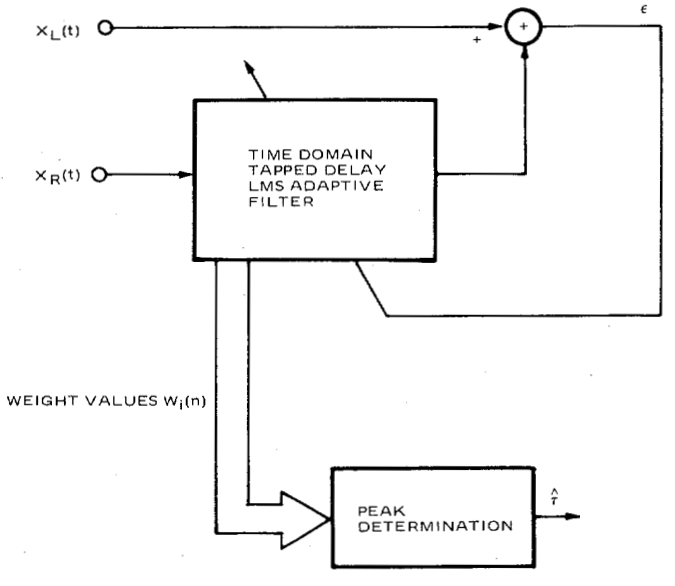
\includegraphics[width=0.5\textwidth]{figures/LMS.png}
	\end{center}
	\caption{TDE using an LMS filter}
	\label{fig:LMS}
\end{figure}


\subsection{Adaptive Eigenvalue Decomposition}
Adaptive eigenvalue decomposition (AED) algorithm was proposed to deal with TDE in reverberant environments. Unlike the crosscorrelation stated above, this algorithm first identifies the channel impulse responses from the source to the two sensors. The delay estimate is then determined by finding the direct paths from the two measured impulse responses. To do that, we observe that
\begin{dmath}
  x_2[k] * g_1 = s[k] * g_2 * g_1 = x_1[k] * g_2
\end{dmath}
  
  Then, we can state that $R_u = 0$. This implies that vector $u$ which consists of two impulse responses is in the null space of R. More specifically, $u$ is the eigenvector of $R$ corresponding to the eigenvalue 0 ($u[k]=g_2[k] - g_1[k]$). We observe that $u$ can be uniquely determined if the following two conditions hold \cite{overview, aed}:
\begin{itemize}
  \item $g_1$ and $g_2$ do not share any common zeros.
  \item The covariance matrix $R$ is full rank.
\end{itemize}

  In case of noise, the covariance matrix will regularize. That will provoke that the algorithm stated above become inoperable because the lack of a 0 eigenvalue. To solve that we have implement this adaptive algorithm that calculate the eigenvector with minimum eigenvalue:
 \begin{dmath}
    u[k+1] = \frac{u[k] - \mu e[k] x[k]}{||u[k]||}
 \end{dmath}
 where $\mu$ is the positive adaptation step.
 

  With the identified impulse responses $g_1$ and $g_2$, the time delay estimate is determined as the difference between two direct paths. That is $T_{\text{AED}} = \arg\max_T |g_2|-|g_1|$. 

  Finally, the noise will not be a problem with the time delay estimation because we only want to find the two direct path and not the whole impulse response. Then, AED is the best of the stated algorithms in front of noise and reverberation. 

  
\section{Preconditioning filters}
  Prior to the delay detection, it is not only useful, but also necessary, to preprocess the filter in some way. Usually, TDE block gets confused by noise, reflections and variance in the power throughout time. Each preconditioning method tries to solve these problem.
\subsection{Time Gain Normalization}
  Time Gain Normalization algorithm tries to fit the average amplitude to a fixed level, by calculating the long-term average level $\overline{x}[n]$ using a smoothing time averaging parameter $\alpha$ and a $L^P$ norm the following way:
  $$ \overline{x[n]} = (\alpha \overline{x}^P[n-1] + (1-\alpha) |\overline{x}[n]|^P ) ^{\frac{1}{P}} $$
  
  So, the output signal with normalized gain $r^2$ can be computed as
  $$ x_{norm}[n] = r \frac{x[n]}{\overline{x}[n-1]} $$
  
  The implementation of Time Gain Normalization can be seen in file \emph{time\_gain.m}\cite{timegain}.
  
\subsection{Spectral Substraction}
  Spectral subtraction is a method for restoration of the power spectrum or the magnitude spectrum of a signal observed in additive noise, through subtraction of an estimate of the average noise spectrum from the noisy signal spectrum. The noise spectrum is usually estimated, and then updated from the periods when the signal is absent and only the noise is present. We did the assumption that the noise is a stationary or a slowly varying process, and that the noise spectrum does not change significantly between the update periods \cite{speech}. 

  For restoration of time-domain signals, an estimate of the instantaneous magnitude spectrum is combined with the phase of the noisy signal, and then transformed via an inverse discrete Fourier transform to the time domain. 

  In terms of computational complexity, spectral subtraction is relatively inexpensive. The magnitude and power spectrum are non-negative variables, and any negative estimates of these variables should be mapped into non-negative values. This nonlinear rectification process provoke a distortion in the cleaned signal. The processing distortion becomes more noticeable as the signal-to-noise ratio decreases. To diminish the distortion due to the harder spectrum attenuation, we have added the spectral floor (Beta) to limit the subtraction and force some residual noise in the output.
  
  We can observe the algorithm with the spectral floor:
  $$
  |X|^2 = \left\{  \begin{array}{rl}
    |Y|^2-\alpha |N|^2    &\mbox{ if  $|X|^2>\beta |N|^2$ } \\
    \beta |N|^2   &\mbox{ otherwise } 
  \end{array} \right.
  $$
  
  Where $X$ is the spectrum of the clean signal, $Y$ is the noise signal, $N$ is the estimated noise spectrum, $\alpha$ is the oversubtraction parameter and $\beta$ is the spectral floor.
  
  The implementation of Spectral Substraction can be seen in file \emph{spectralsubstraction.m}\cite{timegain}.

\subsection{Percentile Noise Removal}
  Percentile Noise removal is a method for restoration of the power spectrum through substraction of an estimate of the percentile nth of the noise spectrum from the noisy signal spectrum. The noise spectrum is usually estimated like in the spectral subtraction method. Then, we apply the percentile function to this noise spectrum. All of this steps are updated from the periods when the signal is absent and only the noise is present. Finally, we subtract the product of the percentile estimation with a constant to the Spectrogram of the signal. The value of the constant has been fixed to 5 because is the optimum in terms of SNR.

  We did the assumption that the noise is a stationary or a slowly varying process, and that the noise spectrum does not change significantly between the update periods. The magnitude and power spectrum are non-negative variables, and any negative estimates of these variables should be mapped into 0. 

  To proposed percentile value is 90. It has been elected because of is the optimum value and where the curve of spectrogram-percentile is flattest. Note that if we put nth=50, the Percentile Noise Removal is more or less the same algorithm than Spectral Subtraction, since the nth=50 means to do the median of the estimated noise spectrum and the Spectral Subtraction use the average of the noise spectrum.
  
  Here we can observe the PNR algorithm:
  $$ S(t,f)'= max\{S(t,f)- c_{\text{N90}},0\} $$
  where $S(t,f)'$ is the spectrogram of the clean signal, $S(t,f)$ is the spectrogram of the noisy signal, $c$ is the oversubtraction parameter and N90 is the 90 percentile of the estimated noise spectrogram.
  
  The implementation of Percentile Noise Removal can be seen in file \emph{percentile.m}\cite{percentile}.


\section{Experimental Setup}
  \subsection{Origin of the data}
  The data and information is coming from PMRF, an instrumented US Navy testing range located off the island of Kauai, Hawaii. Data were collected from seven bottom mounted hydrophones (4 to 5 m off the seafloor) in deep water (nominally 4,600 meters) approximately 45 km northwest of Kauai. The relative location of the hydrophones, their designations and filenames for the data files are as shown in Table \ref{tab:hydrophones_positions}. Our targets were always minke whales.
  
  \begin{table}
    \caption{Position of hydrophones}
    \label{tab:hydrophones_positions}
  
    \begin{center}
      \begin{tabular}{| l | l | l | l | l |}
         \hline
         hydrophone \# & X[m] & Y[m] & Z[m]  & filename \\ \hline
         7 \# & -6129 & 9784 & -4750  & 27Apr09\_074921\_NN\_p7.wav \\ \hline
         6 \# & -6183 & -4874 & -4650  & 27Apr09\_074921\_NN\_p6.wav \\ \hline
         5 \# & -6163 & -12402 & -4600  & 27Apr09\_074921\_NN\_p5.wav \\ \hline
         4 \# & 6865 & 12844 & -4750  & 27Apr09\_074921\_NN\_p4.wav \\ \hline
         3 \# & 6520 & 5240 & -4650  & 27Apr09\_074921\_NN\_p3.wav \\ \hline
         2 \# & 6635 & -2132 & -4500  & 27Apr09\_074921\_NN\_p2.wav \\ \hline
         1 \# & 6566 & -9617 & -4500  & 27Apr09\_074921\_NN\_p1.wav \\ \hline
      \end{tabular}
    \end{center}
  \end{table}
  
  The dataset is from the 27th of April 2009 at approximately 12:00 Hawaiian standard time. Thirty minutes of data from each hydrophone are provided as three files (approx. 10 minutes per file). The sampling rate of the recordings (Windows PCM .wav format) is $Fs=\SI{96}{\kilo\Hz}$ with 16 bits resolution. The data are sampled simultaneously, so sample N from one file is the same relative time as sample N of a second file with the same filename. The file format is .wav in little-endian format.
  
  The test signals used to assess the proper implementation of the algorithms were two chirps, two pure tones and white noise delayed a desired number of samples. The implementation of their creation can be seen in file \emph{init\_test\_signals.m}\cite{inittestsignals.m}.
  
\subsection{Procedure}
  First two signals are loaded and cut them to focus at an interesting event. We've used Audacity to discover the minke whale sounds. Knowing that the first event of the sensor 1 is at 2:35 and the position of the sensors, we choose a window of signal of $2 TDOA_{max}$. $TDOA_{max}$ is the maximum possible delay between to pair of microphones, that is, $\frac{\text{distance}}{c}$, where $c$ is the speed of sound underwater. The worst case is when the delay is computed between the furthest microphones. Such value has been computed using code in file \cite{maxdelay.m}. $c$ is always considered constant, altough better approximations could have been used, taking into consideration temperature, salinity and pressure (depth) \cite{speed-sound-seawater}. Due the huge distance between sensors (many kilometers), such window is around 20-25 s. This will a problem when we run the adaptive algorithms.

  Then, after having cut the signal, we pre-processed it with a noise removal algorithm. Finally, we do the TDE between the two signals. Knowing the true delay, we only have to do a ground truth assess. Then, we record the results as relative error and absolute error in samples. We have done the simulations with sensors 1, 2, 3, 4 and 5 with interesting results.

\subsection{Some events}
  Taking as a reference microphone 2, we focused on two events:
  \begin{itemize}
    \item First event: 2:20-2:45. Only noise, no other interference than the constant tone at much higher frequencies.
    \item Second event: 8:40-9:00. It has interferences from other animals (dolphins and whales). For this reason, it's more critical and more important to reduce strongly the noise and interference. The results of the simulation depend heavily on the algorithms of noise reduction and TDOA used.
  \end{itemize}

  
\section{Results}
  In this section, the results of the successfuly implemented methods that perform better will be shown. That means the combination of preconditioning filters and the TDE algorithm and their parameters.

\subsection{Prefiltering methods}
First, as it is a crucial step, the prefiltering methods are assessed individually.

\subsubsection{PNR}

  \begin{figure}[htb]
	  \begin{center}
		  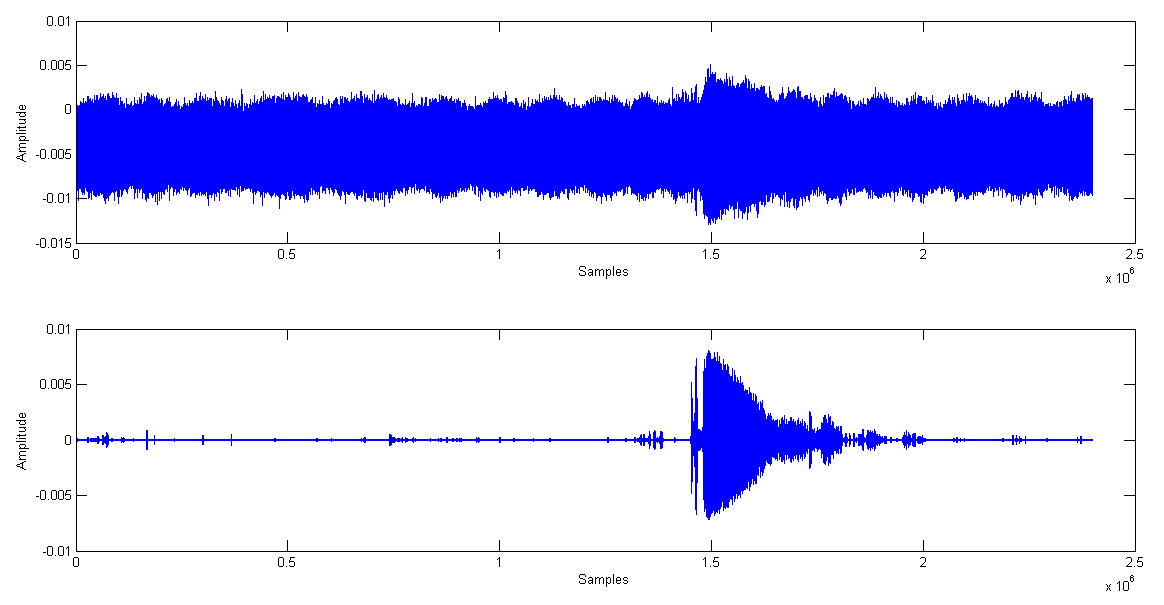
\includegraphics[width=0.5\textwidth]{figures/1PNR_waveform.png}
	  \end{center}
	  \caption{Above: Waveform of sensor 1 recording without pre-processing. Below: Waveform of sensor 1 recording after filter + PNR}
	  \label{fig:result_PNR_waveform}
  \end{figure}

  In the Figure \ref{fig:result_PNR_waveform}, at the top we can see the noisy signal and at the bottom the signal after being processed with Percentile Noise removal. We can observe that the algorithm has deleted almost all of the noise. However, the signal has decreased its level.

  After assessing the improvement, we can state that the SNR before the pre-processing was \SI{3.06}{\dB} and after applying the band pass filter and PNR, it increased up to \SI{39.50}{\dB}. This leads to a good noise reduction algorithm. Computing the entropy using the built-in MATLAB funcion \emph{entropy()}, the result is that after the pre-processing the entropy value increases. This is not what we would have expected a priori. The reason is that we have subtracted the correlated noise and pre-whitened the signal. Therefore, we have added a little randomness in the final signal. That is why entropy is not always a good assessment method. However, visually it enhances a lot the scenario and the TDE performs with much more accuracy.
  
  \begin{figure}[htb]
	  \begin{center}
		  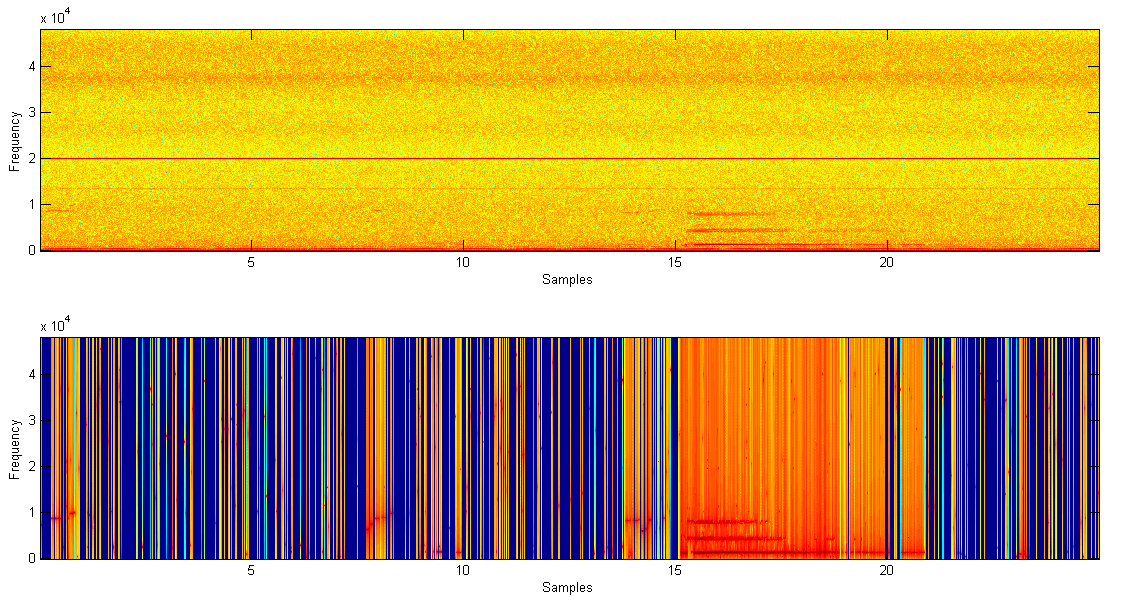
\includegraphics[width=0.5\textwidth]{figures/2PNR_spec.png}
	  \end{center}
	  \caption{Above: Spectrogram of sensor 1 recording without pre-processing. Below: Spectrogram of sensor 1 recording after filter + PNR}
	  \label{fig:result_PNR_spec}
  \end{figure}

  At Figure \ref{fig:result_PNR_spec} we can see the noisy spectrogram and the "clean" spectrogram after being processed with PNR. We can observe that the algorithm has modified completely the Spectrogram. After a lot of work done in the implementation of the algorithm, we could not be able to improve the spectrogram. A missing issue about this algorithm is that there was not enough time to find the optimal parameters: window length and window length shift. This might have improved the visual aspect of the spectrogram. Furthermore, the distance between sensors and the computational complexity of the algorithm made the work harder. However, after simple visual inspection, it's easier to identify the whale sound in the spectrogram, as the SNR of the clean signal has increased.
  

\subsubsection{Spectral Substraction}
  
  \begin{figure}[htb]
	  \begin{center}
		  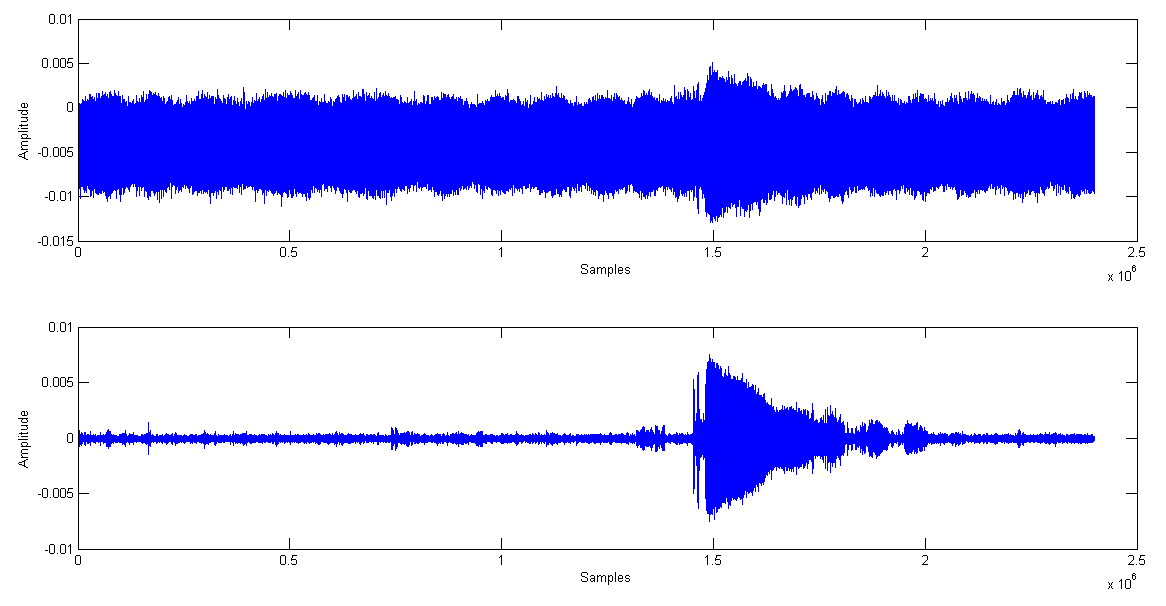
\includegraphics[width=0.5\textwidth]{figures/3SpectralSub_waveform.png}
	  \end{center}
	  \caption{Above: Waveform of sensor 1 recording without pre-processing.  Below: Waveform of sensor 1 recording after filter + Spectral Substraction}
	  \label{fig:result_SS_waveform}
  \end{figure}
  
  Figure \ref{fig:result_SS_waveform} shows the noisy signal and the signal after being processed with Spectral Subtraction. We can observe that the algorithm has deleted most of the noise although the signal has decreased it level a little bit. It doesn't decrease all the noise because of the parameter $\beta$, which fixes a noise floor.
  After assessing the improvement, we can state that the SNR before the pre-processing was \SI{3.0583}{\dB} and after applying the band pass filter + SS, it increased up to \SI{33.88}{\dB}. The same reasoning as in PNR case can be made. The enhancement is a little bit lower but still very high. This is because SS is a particularization of PNR when the percentile value is 50.

  \begin{figure}[htb]
	  \begin{center}
		  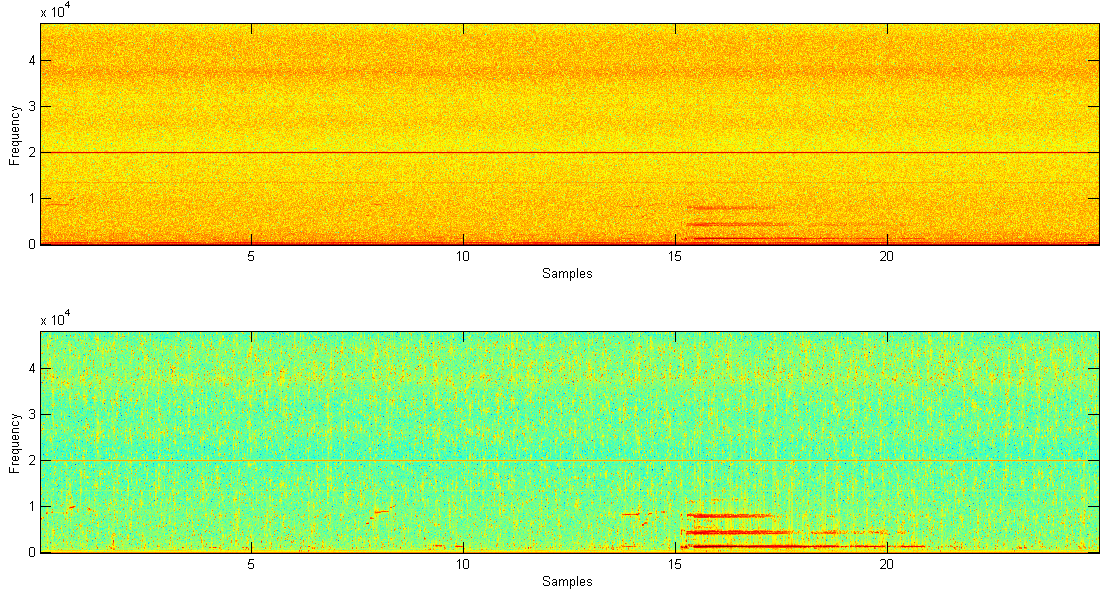
\includegraphics[width=0.5\textwidth]{figures/4SpectralSub_Specgram.png}
	  \end{center}
	  \caption{Above: Spectrogram of sensor 1 recording without pre-processing.  Below: Spectrogram of sensor 1 recording after filter + Spectral Substraction}
	  \label{fig:result_SS_spec}
  \end{figure}
  
  Figure \ref{fig:result_SS_spec} shows the noisy signal and the signal after being processed with Spectral Subtraction. We can observe that the algorithm has a much more good-looking Spectrogram than in PNR method, but the SNR is lower. This could be due to the parameter $\beta$, that allows a little noise level in the clean signal. In TDE, the PNR performs better because, although the clean signal has more distortion, it is looking at the peak to find the correlation between sensors. Then, for our application, we will have better results pre-processing with the PNR rather than with Spectral Subtraction Algorithm.
  
\subsection{TDE}
  With Time Gain Normalization algorithm, we observe quite good results in Time Delay Estimation. All the situations have a relative error below 1\% despite one simulation that has a relative error of 500\% (GCC-SCOT between sensors 1-2. at 2nd Event).
  With Percentile Noise Removal denoising algorithm, the results in Time Delay Estimation outperform. Indeed, all the simulations have a relative error below 0.7\%. If we apply the band-pass filter, we keep obtaining the same results.
  Finally, with Spectral Subtraction algorithm we observe bad results in Time Delay Estimation. Indeed, all the simulations with GCC-PHAT and almost all of them with GCC-SCOT get a relative error of 100\%. If we apply the band pass filter, we keep obtaining good results with the cross-correlation (below 1.5\% of relative error) and we have improved the simulations with PHAT and SCOT. However, PHAT algorithm keep getting a relative error of 50\%.
  As stated before, the cross-correlation algorithm presents good results in all the possible simulations. The interpretation of this results can be understood as the problem of Time Gain Normalization. This is that the high distance between the sensors leads to a small coherence between the received signals, so it makes the PHAT algorithm weak. About the failure of the SCOT without applying the filter can be explained as the Scot algorithm has taken into account the coherence between the strong interference at \SI{20}{\kilo\Hz} in sensors 3 and 4. Then, applying the filter we eliminate that interference.
  We sum up saying that PNR is the best noise reduction algorithm we have explained. We had expected this result when getting \SI{39.5}{\dB} of SNR stated previously.
  
    \subsubsection{GCC-SCOT with PNR}

      \begin{figure}[htb]
	      \begin{center}
		      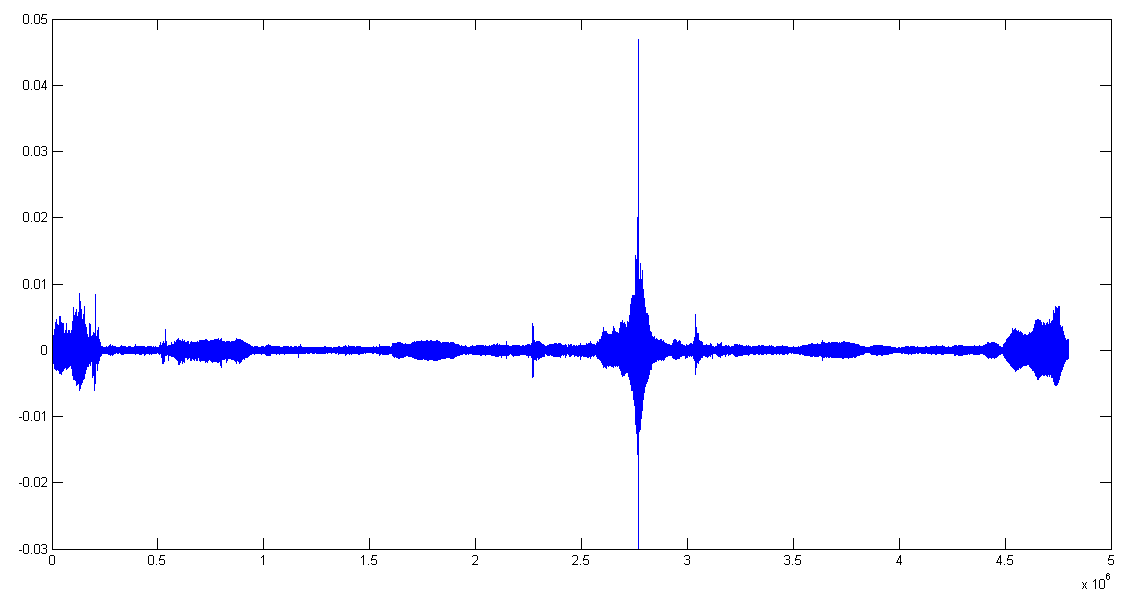
\includegraphics[width=0.5\textwidth]{figures/5gcc_Scot_PNR_12_1.png}
	      \end{center}
	      \caption{GCC-SCOT between sensors 1 and 2 at the first event (2:20-2:45) after PNR}
	      \label{fig:result_GCC_SCOT}
      \end{figure}
      
      Figure \ref{fig:result_GCC_SCOT} shows GCC-SCOT between sensors 1 and 2 at the first minke whale event. As we were expecting after looking at the SNR stated above, the Time Delay Estimation is very accurate. Indeed, we have only a 0.26\% of relative error. GCC-SCOT regularly performs that better. Simulations between sensors 1 and 2, 3, 4 and 5 at the two events and pre-processing with the Percentile Noise Removal algorithm, all of them obtained less than 0.7\% of relative error in all the simulations. We have tried the simulations with these algorithms: Cross-correlation, SCOT Generalised Cross-correlation and PHAT Generalised Cross-correlation.
  
    \subsubsection{GCC-PHAT with Spectral Substraction}
    
    \begin{figure}[htb]
      \begin{center}
	      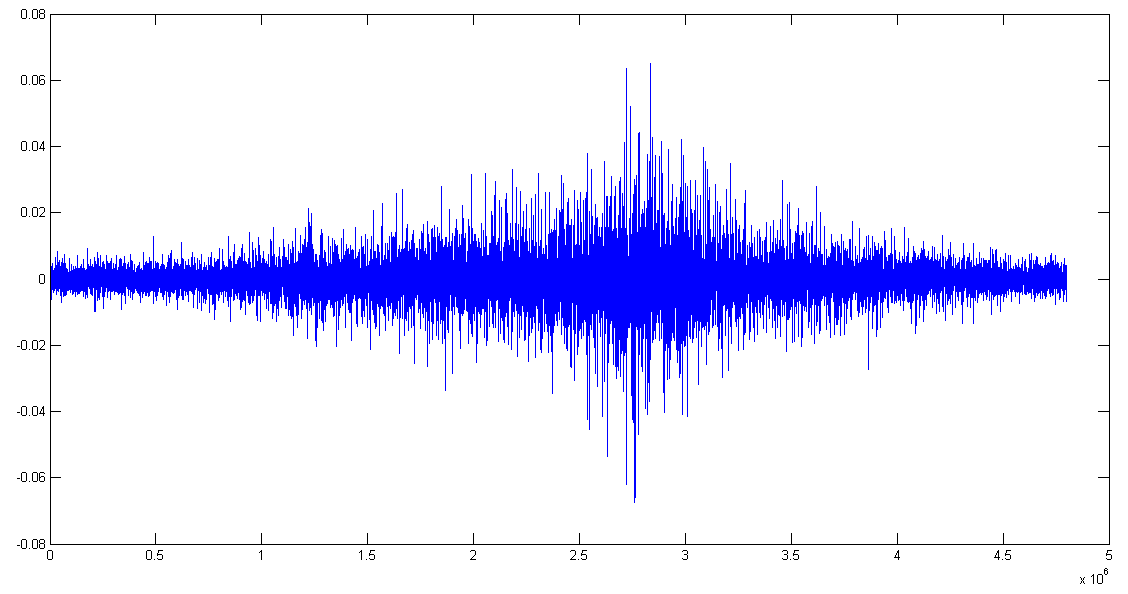
\includegraphics[width=0.5\textwidth]{figures/6gcc_Phat_SS_12_1.png}
      \end{center}
      \caption{GCC-PHAT between sensors 1 and 2 at the first event (2:20-2:45) after Spectral Substraction}
      \label{fig:result_GCC_PHAT}
    \end{figure}
      
    Figure \ref{fig:result_GCC_PHAT} shows GCC-PHAT between sensors 1 and 2 at the first minke whale event. Looking at the plot, we can see that the Time Delay Estimation is quite poor. Indeed, we got relative error of 18\%. PHAT algorithm doesn't work well in all the simulations. Due to the high (12-28 km) distance between the sensors, the coherence of the received signals is very low. While SCOT takes that into account, the PHAT algorithm fails in some of these situations. The PNR is the only noise removal algorithm that leads to a good GCC-PHAT results in all the simulations.

  
\section{Localization}
  Given a time delay and the known position of the sensors, a loci of possible points of the source gets defined. For each pair of sensors, an hyperbola of possible points is defined. For a given estimated delay of $\tau_{ij}$ between two sensors located at $(x_i,y_i,z_i)$ and $(x_j,y_j,z_j)$ and for a constant speed of sound of $c$, the resulting hyperbola is represented at Figure \ref{fig:hyp} and its expression is
\begin{dmath}
  \tau_{ij} = \frac{1}{c}\left(\sqrt{(x-x_i)^2 + (y-y_i)^2 + (z-z_i)^2} - 
  \sqrt{(x-x_j)^2 + (y-y_j)^2 + (z-z_j)^2} \right)
\end{dmath}

\begin{figure}[htb]
	\begin{center}
		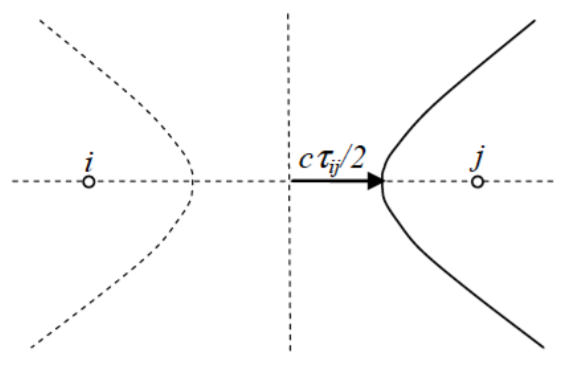
\includegraphics[width=0.4\textwidth]{figures/tdoa.png}
	\end{center}
	\caption{2D hyperbola loci defined for a TDOA of $\tau_{ij}$ between sensors $i$ and $j$}
	\label{fig:hyp}
\end{figure}

So, later on, with another pair of microphones, the intersection yields to the source localization.

In our short experiment, for tracking a minke whale on a 2D map, we have developed a rudimentary multilateration system, on the basis of 6 TDOAs only. The localization by itself leads to a non-linear solution. In addition, non-idealities imply a no unique solution, so we get a zone where the source could be located. We have not gone so far, but the estimated position could have been estimated by algorithms such as Crossing Lines or Steered-response power.

We first show the position of the hydrophones on the map, and then plot the hyperbolas corresponding to each pair of TDOA, assuming the speed of sound in water is 1510 m/s \cite{speed-sound-seawater}.  We have computed the TDOA between the sensor 1 and all the other ones, after having pre-processed the signals with PNR and doing the estimation with the Generalised Cross-Correlation Smoothed Coherence Transform.

\begin{figure*}[htb]
	\begin{center}
		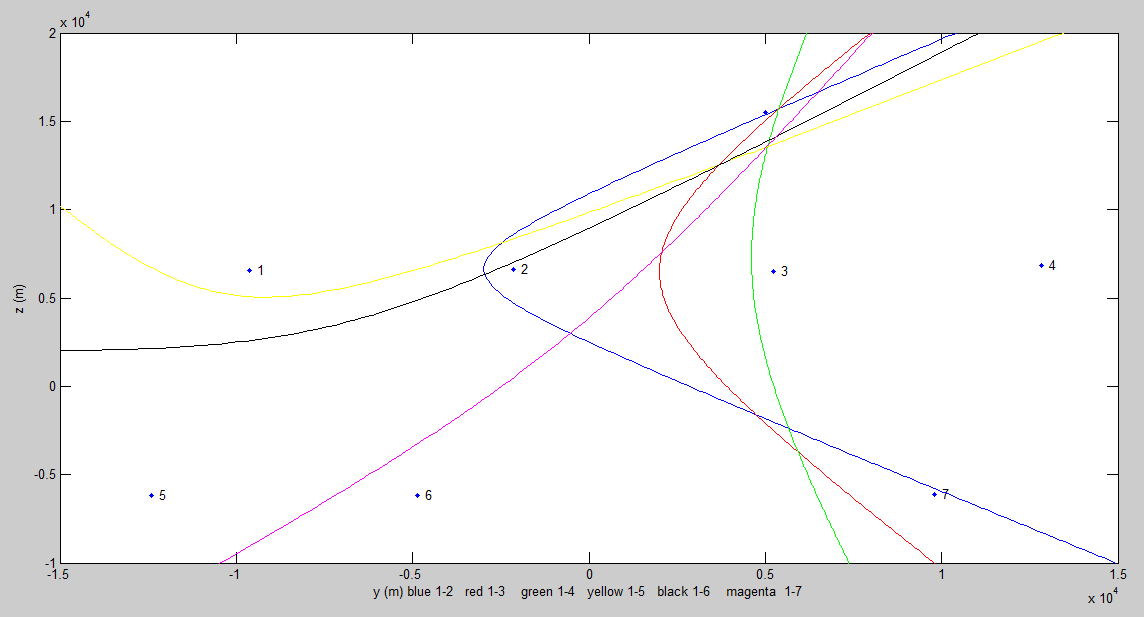
\includegraphics[width=1\textwidth]{figures/7_local.png}
	\end{center}
	\caption{Localization of the minke whale through multilateratization between sensor 1 and the rest.}
	\label{fig:local}
\end{figure*}

Then, looking at Figure \ref{fig:local}, we have obtained 7 curves that ideally will intersect at one point. In our case, it is quite normal that the curves don't intersect all, but we can see where the whale is approximately, as the curves intersect in a little area. The first 5 curves have a Time Delay Estimation error smaller than 1\%. The worst case corresponds to the furthest sensors, 1 and 7, and they are separated \SI{28}{\kilo\meter}, so our resolution is \SI{280}{\meter}. That is why the curves don't match in one point. Nevertheless, we do a rough visual estimation so the whale is at the position x=13700 y=5300.


\section{Graphical User Interface}
  The Graphical User Interface, built using the GUIDE MATLAB tool, has all the capabilities stated at the Introduction, section B, "Scope of the project".

An screenshot of the same can be seen at Figure \ref{fig:GUI} using the GCC-SCOT result with Time Gain Normalization. The two loaded signals come from sensors 1 and 2 and are focused at the minke whale sound \#1 (a Minke whale sound).

The 3D distribution of the PMRF sensors can be seen and rotated using the option View 3D position of sensors. A screenshot is attached at Figure \ref{fig:3D_sensors}. The corresponding code is in file \emph{plot3Dsensors.m} \cite{plot3Dsensors.m}.

The code of the GUI is in file \emph{interactive\_TDE.m}\cite{interactiveTDE.m} and \emph{localization.m}\cite{localization.m}.

\begin{figure*}[!t]
	\begin{center}
		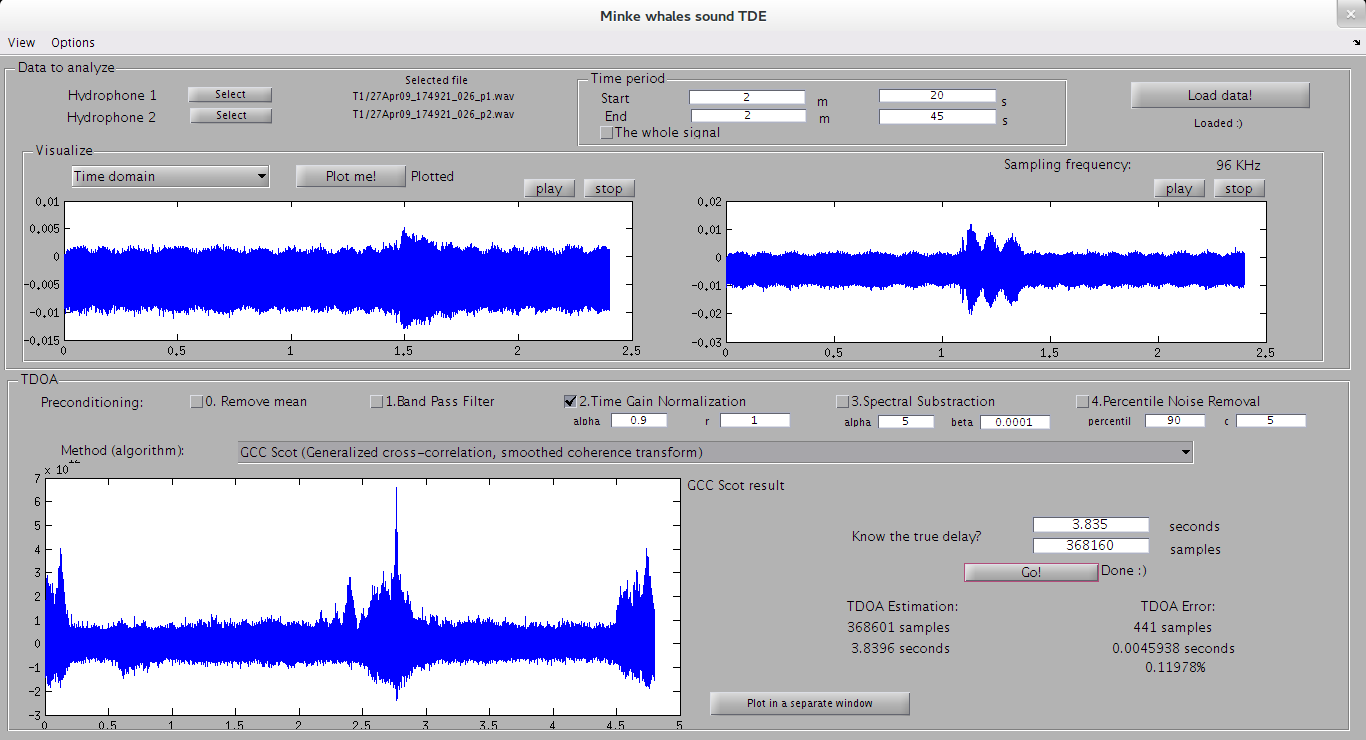
\includegraphics[width=1\textwidth]{figures/GUI_SCOT.png}
	\end{center}
	\caption{Graphical User Interface screenshot with a GCC-SCOT estimation using Time Gain Normalization over a Minke Whale sound}
	\label{fig:GUI}
\end{figure*}

\begin{figure}[htb]
	\begin{center}
		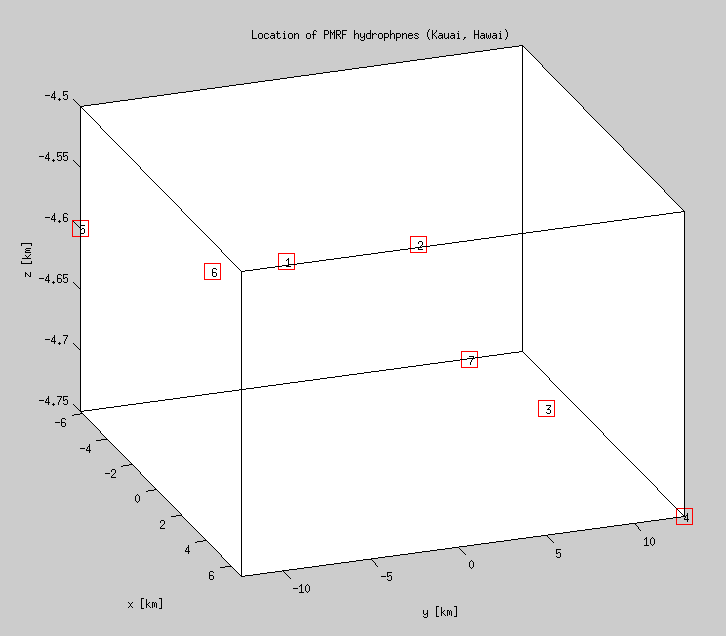
\includegraphics[width=0.5\textwidth]{figures/3D_sensors.png}
	\end{center}
	\caption{Underwater distribution of the PMRF hydrophones in kilometers}
	\label{fig:3D_sensors}
\end{figure}

  
\section{Code}
  All the code of the project is publicy available in a git repository on Bitbucket within the next URL: \url{https://bitbucket.org/javiribera/tde-and-whale-localization/src}
A brief high-level explanation of some files is done below:
\newpage

\begin{itemize}
  \item \emph{algorithms\_TDE} folder
    \begin{itemize}
      \item \emph{gcc.m} \cite{gcc.m} computes the Generalized Cross-Correlation between parameter 1 and 2 using the weighting algorithm passed as third parameter ("cc","phat" or "scot").
      \item \emph{delay\_gcc.m} \cite{delaygcc.m} bypasses its parameters to \emph{gcc.m} and takes the last maximum index value.
      \item \emph{delay\_xcorr.m} \cite{delayxcorr.m} computes the classical cross-correlation and also takes the last maximum index value.
      \item \emph{delay\_lms.m} \cite{delaylms.m} returns the delay between first and second parameter using LMS adaptive method using the fifth parameter (beta) as smoothing parameter. The third (max\_expected) and forth (length\_signal) parameters are used to know the minimum order or the filter. The last parameter (handles) is used only to be able to plot the results to the GUI.
    \end{itemize}
    
  \item \emph{preconditioning} folder
    \begin{itemize}
      \item \emph{build\_filter.m} \cite{buildfilter.m} returns a very high-order (50) filter designed to bandpass filter minke whale sounds (1 and \SI{12}{\kilo\Hz}).
      \item \emph{filter\_passband.m} \cite{filterpassband.m} outputs the input after being filtered by the filter returned by \emph{build\_filter.m}.
      \item \emph{percentile.m} \cite{percentile.m} outputs the input after being processed by the percentile noise removal algorithm.
      \item \emph{spectralsubstraction.m} \cite{spectralsubstraction.m} outputs the input processed by the spectral substraction algorithm.
      \item \emph{time\_gain.m} \cite{timegain.m} outputs the input after being processed by the Time Gain Normalization algorithm.
    \end{itemize}
    
  \item \emph{GUI} folder
    \begin{itemize}
      \item \emph{main\_GUI.m} \cite{mainGUI.m} is a simple 2-button GUI to choose between the next 2 GUI:
      \item \emph{interactive\_TDE.m} \cite{interactiveTDE.m} displays the GUI shown at Figure \ref{fig:GUI} that has all the capabilities explained at Introduction, section B, "Scope of the project".
      \item \emph{localization.m} \cite{localization.m} displays the GUI shown at Figure \ref{fig:hyp} that has all the capabilities explained at Introduction, section B, "Scope of the project".
    \end{itemize}
    
  \item \emph{clean\_signal.m} \cite{cleansignal.m} accepts as the second parameter ("preprocessing\_methods") a string cell array containing the names of the preconditioning methods to be applied to the signal in the first parameter ("input"). Available options are:
"remove\_mean", "band\_pass", "time\_gain", "spectral\_substraction", "percentile" and "tk". It applies the selected method in a hardcoded order and outputs the clean signal.
    
  \item \emph{clean\_signal.m} \cite{cleansignal.m} is a script to create the 7x3 matrix containing the [X,Y,Z] position of the hydrophones in meters.
    
  \item \emph{test\_signals/init\_test\_signals.m} \cite{inittestsignals.m} is a script that creates three pairs of artificial signals (two tones, two chirps and 2 random noise signals) identical but delayed a known number of seconds, given a sample frequency. It then saves them inside folder \emph{test\_signals}as a \emph{.mat} file and as \emph{.wav} files.
    
  \item \emph{utils} folder
    \begin{itemize}
      \item \emph{delay\_between\_sensors.m} \cite{delaybetweensensors.m} returns the delay in seconds between the sensors provided by the indexes at first and second parameter.
      \item \emph{plot3Dsensors.m} \cite{plot3Dsensors.m} shows the 3D disposition of the PMRF hydrophones.
      \item \emph{sensors\_delay\_max.m.m} \cite{maxdelay.m} computes the maximum possible delay in seconds between the furthest sensors.
    \end{itemize}
    
\end{itemize}


\section{Conclusions}
  Seen the results, the feasibility of a simple localization has been proved, as long as the proper noise reduction algorithm is chosen. The limited available amount of time didn't allow us to assess more sophisticated algorithms such as LMS and AED. Additionaly, we would have also liked to be able to implement localization algorithms (Crossing Lines and Steered-response power) and to be able to track the evolution of the whale.


\appendices


% use section* for acknowledgement
\section*{Acknowledgment}
  We would like to thank Ludwig Houégnigan for the proposal of this topic for our project, for providing us the data and for deeply assisting us in theorical and implementation aspects. Also, for kindly reviewing this report.




% Can use something like this to put references on a page
% by themselves when using endfloat and the captionsoff option.
\ifCLASSOPTIONcaptionsoff
  \newpage
\fi



% trigger a \newpage just before the given reference
% number - used to balance the columns on the last page
% adjust value as needed - may need to be readjusted if
% the document is modified later
%\IEEEtriggeratref{8}
% The "triggered" command can be changed if desired:
%\IEEEtriggercmd{\enlargethispage{-5in}}

% references section

% can use a bibliography generated by BibTeX as a .bbl file
% BibTeX documentation can be easily obtained at:
% http://www.ctan.org/tex-archive/biblio/bibtex/contrib/doc/
% The IEEEtran BibTeX style support page is at:
% http://www.michaelshell.org/tex/ieeetran/bibtex/
\bibliographystyle{IEEEtran}
\bibliography{bibliography}
% argument is your BibTeX string definitions and bibliography database(s)
%\bibliography{IEEEabrv,../bib/paper}
%
% <OR> manually copy in the resultant .bbl file
% set second argument of \begin to the number of references
% (used to reserve space for the reference number labels box)
%\begin{thebibliography}{1}

%\bibitem{IEEEhowto:kopka}
%H.~Kopka and P.~W. Daly, \emph{A Guide to \LaTeX}, 3rd~ed.\hskip 1em plus
%  0.5em minus 0.4em\relax Harlow, England: Addison-Wesley, 1999.

%\end{thebibliography}



\end{document}


